\section{Datenbank--Schema}

\subsection{Konzeptuelles Datenbankschema: Entity--Relationship Diagramm}

Hier werden die Gegenstände der realen Welt modelliert wie in Abbildung \ref{fig:erd} gezeigt modelliert. Hierbei ist zu beachten, dass die Entität „Frage“ das zentrale Element des Datenmodells darstellt. Die weiteren Entitäten „Antwortmöglichkeit“ bzw. „gegebene Antwort” sind existenzabhängige Entities. Ohne Antwortmöglichkeit kann ohne zugehörige Frage nicht existieren, eine gegebene Antwort macht nur Sinn, wenn es eine entsprechende Antwortmöglichkeit und Frage gibt.

Die Entität „Benutzer“ steht in keiner Beziehung zu den anderen Entitäten, sie wird auch nur für die Eingabe neuer Fragen und Antwortmöglichkeiten, bzw. zur Authentifizierung benötigt.

\begin{figure}[H]
\begin{center}
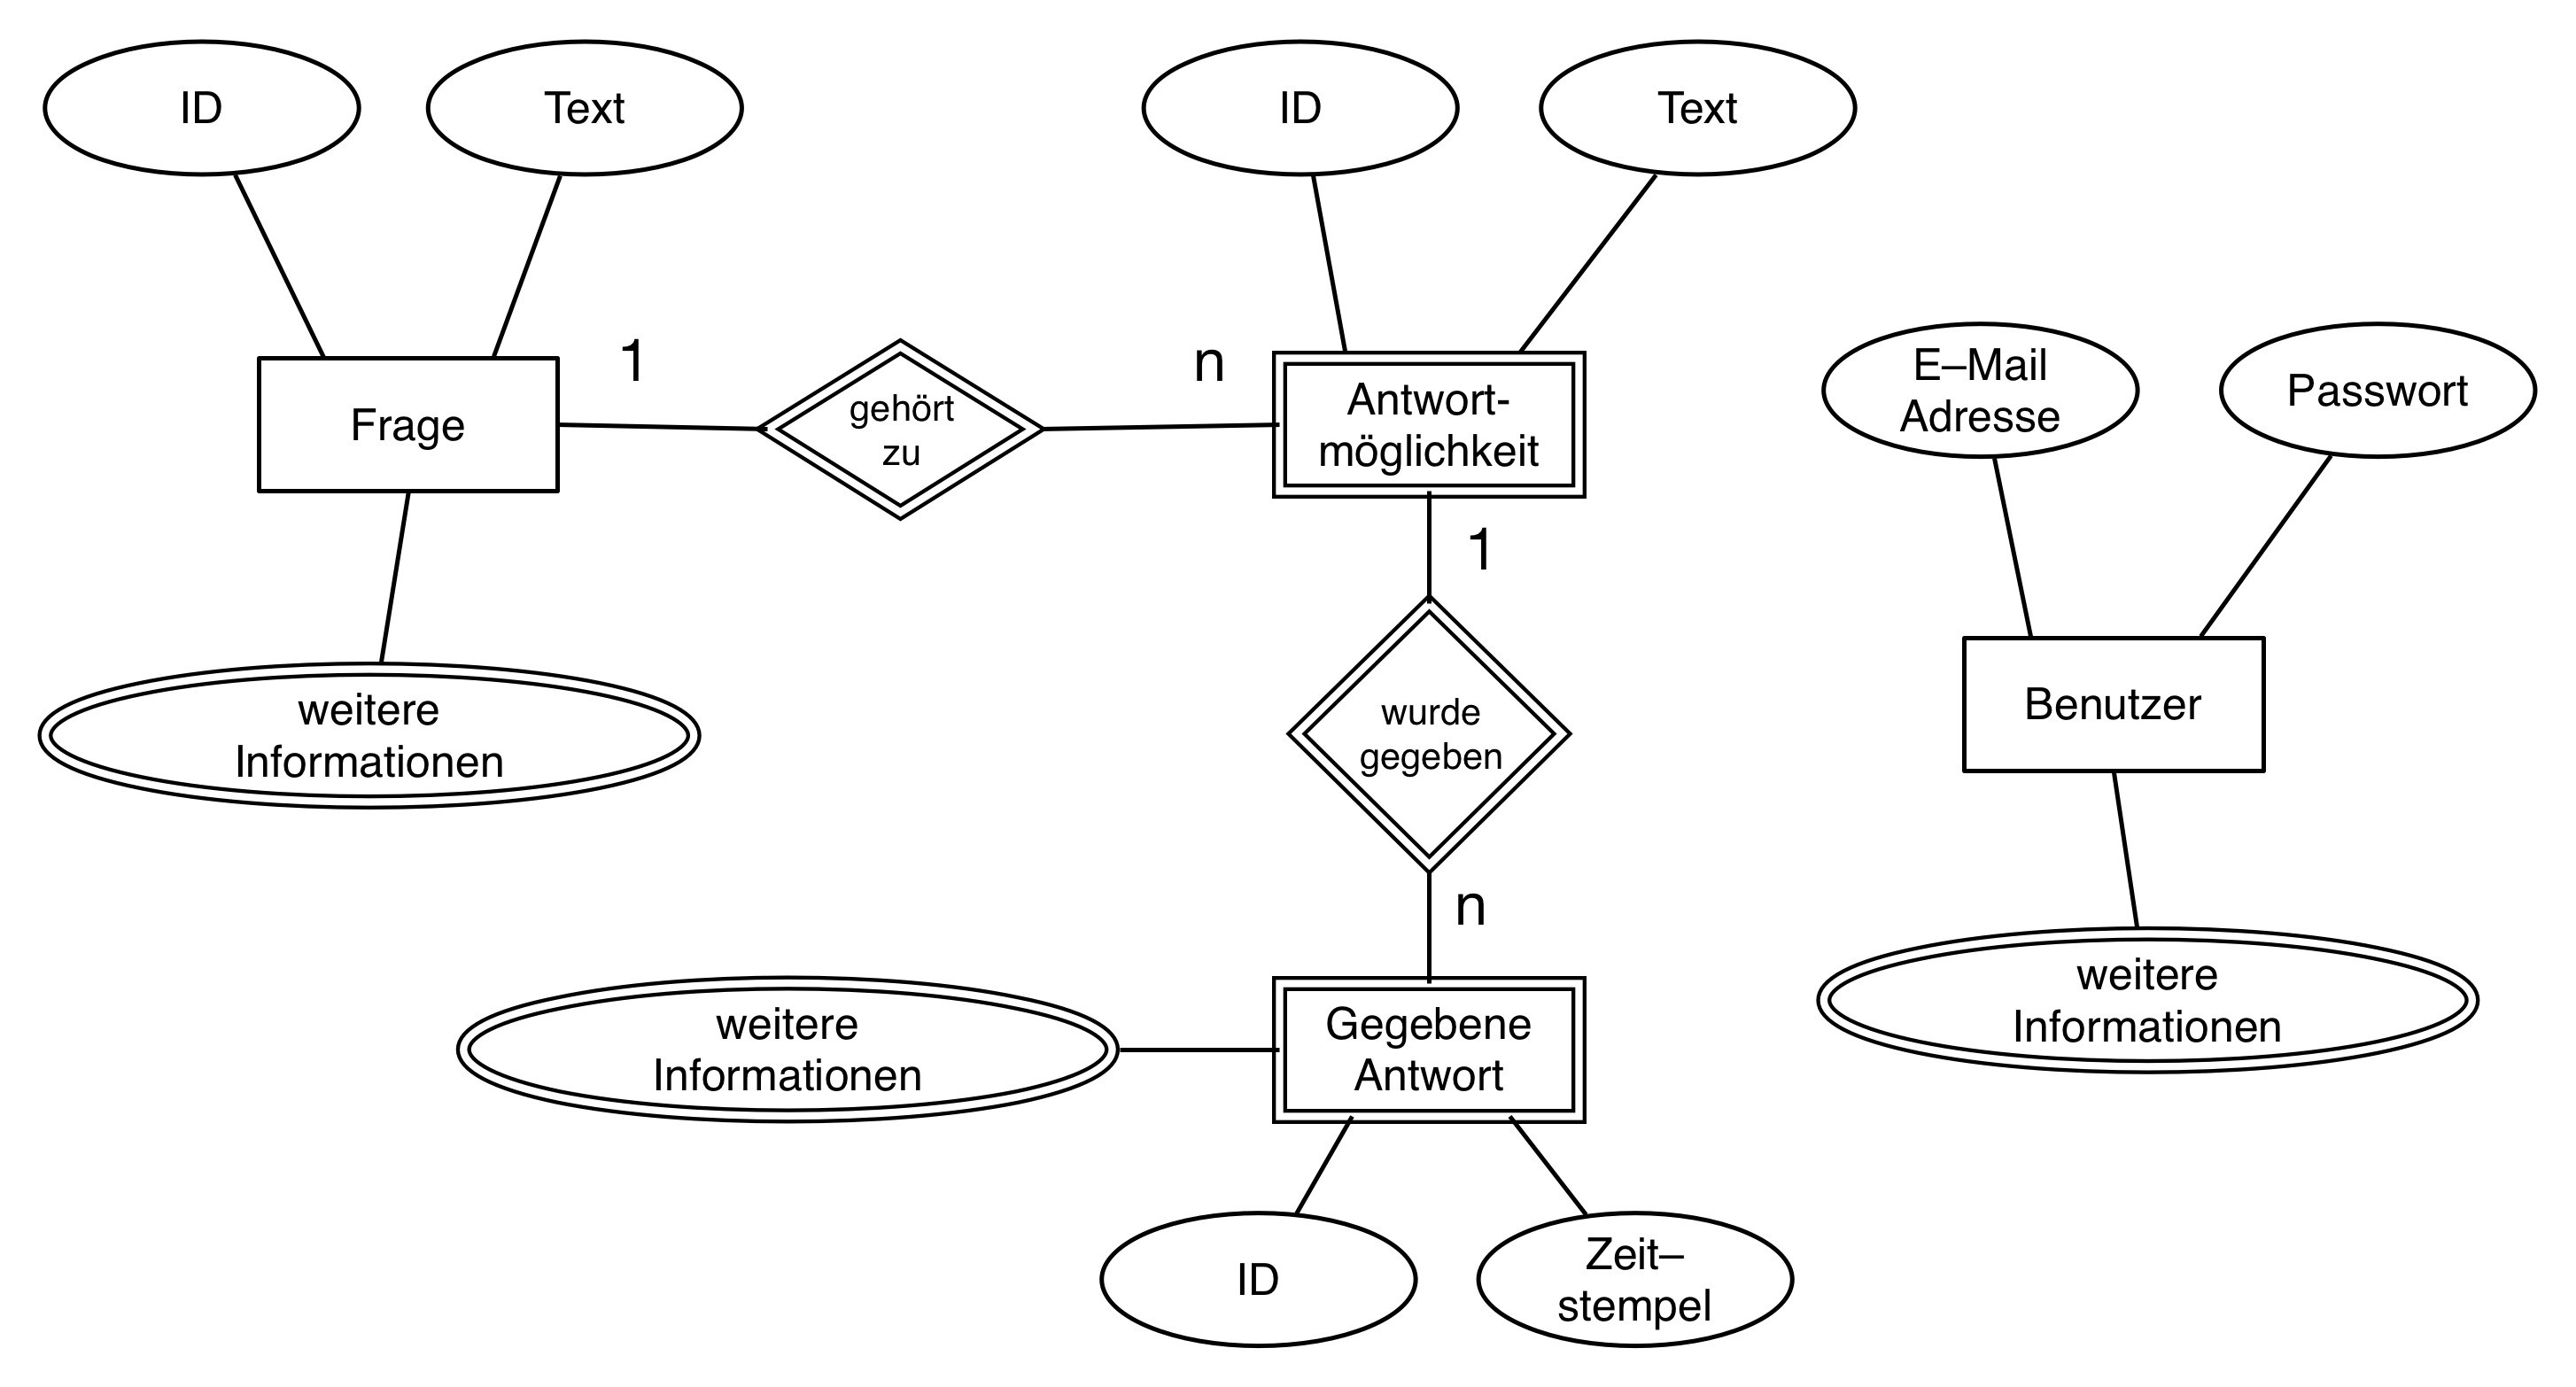
\includegraphics[width=\textwidth]{ERD.jpg}
\caption{Entity Relationship Diagram}
\end{center}
\label{fig:erd}
\end{figure}

Die als zsammengesetzte Attribute dargestellten „weiteren Informationen“ sind Attribute der jeweiligen Entitäten, die für die gestellten Anforderungen nicht notwendig sind, jedoch im Produktivbetrieb großen Zusatznutzen bieten könnten. So wäre es möglich die gegebenen Antworten durch die Speicherung der IP--Adresse, Browser--Fingerprinting\footnote{Die Identifikation eines speziellen Nutzers durch Konfigurationsdetails des Webbrowsers, Bildschirmgröße, Betriebssystemversion, etc. Siehe auch \url{https://panopticlick.eff.org/}} oder andere Techniken genauer zu identifizieren und somit einem bestimmten Nutzer zuzuordnen. Hierbei sind dann die jeweiligen Datenschutzbestimmungen zu beachten.

Die Datensätze der Entity „Frage“ könnten Zeitangaben enthalten, die festlegen wann bzw. wie lange eine Frage auf der Website angezeigt wird. Die Antwortmöglichkeiten könnten durch entsprechende Angaben zur Sortierreihenfolge geordnet werden.

\subsection{Logisches Datenbankschema: Relationales Datenmodell}

Aufgrund des in Abbildung \ref{fig:erd} auf Seite \pageref{fig:erd} dargestelten Modell ergibt sich die in Abbildung \ref{fig:relmod} dargestellten Relationen. Dieses Modell entspricht der 3. Normalform\footnote{Kriterien laut \cite{dao101}, Kapitel 3.4}.

\begin{figure}[H]
\begin{center}
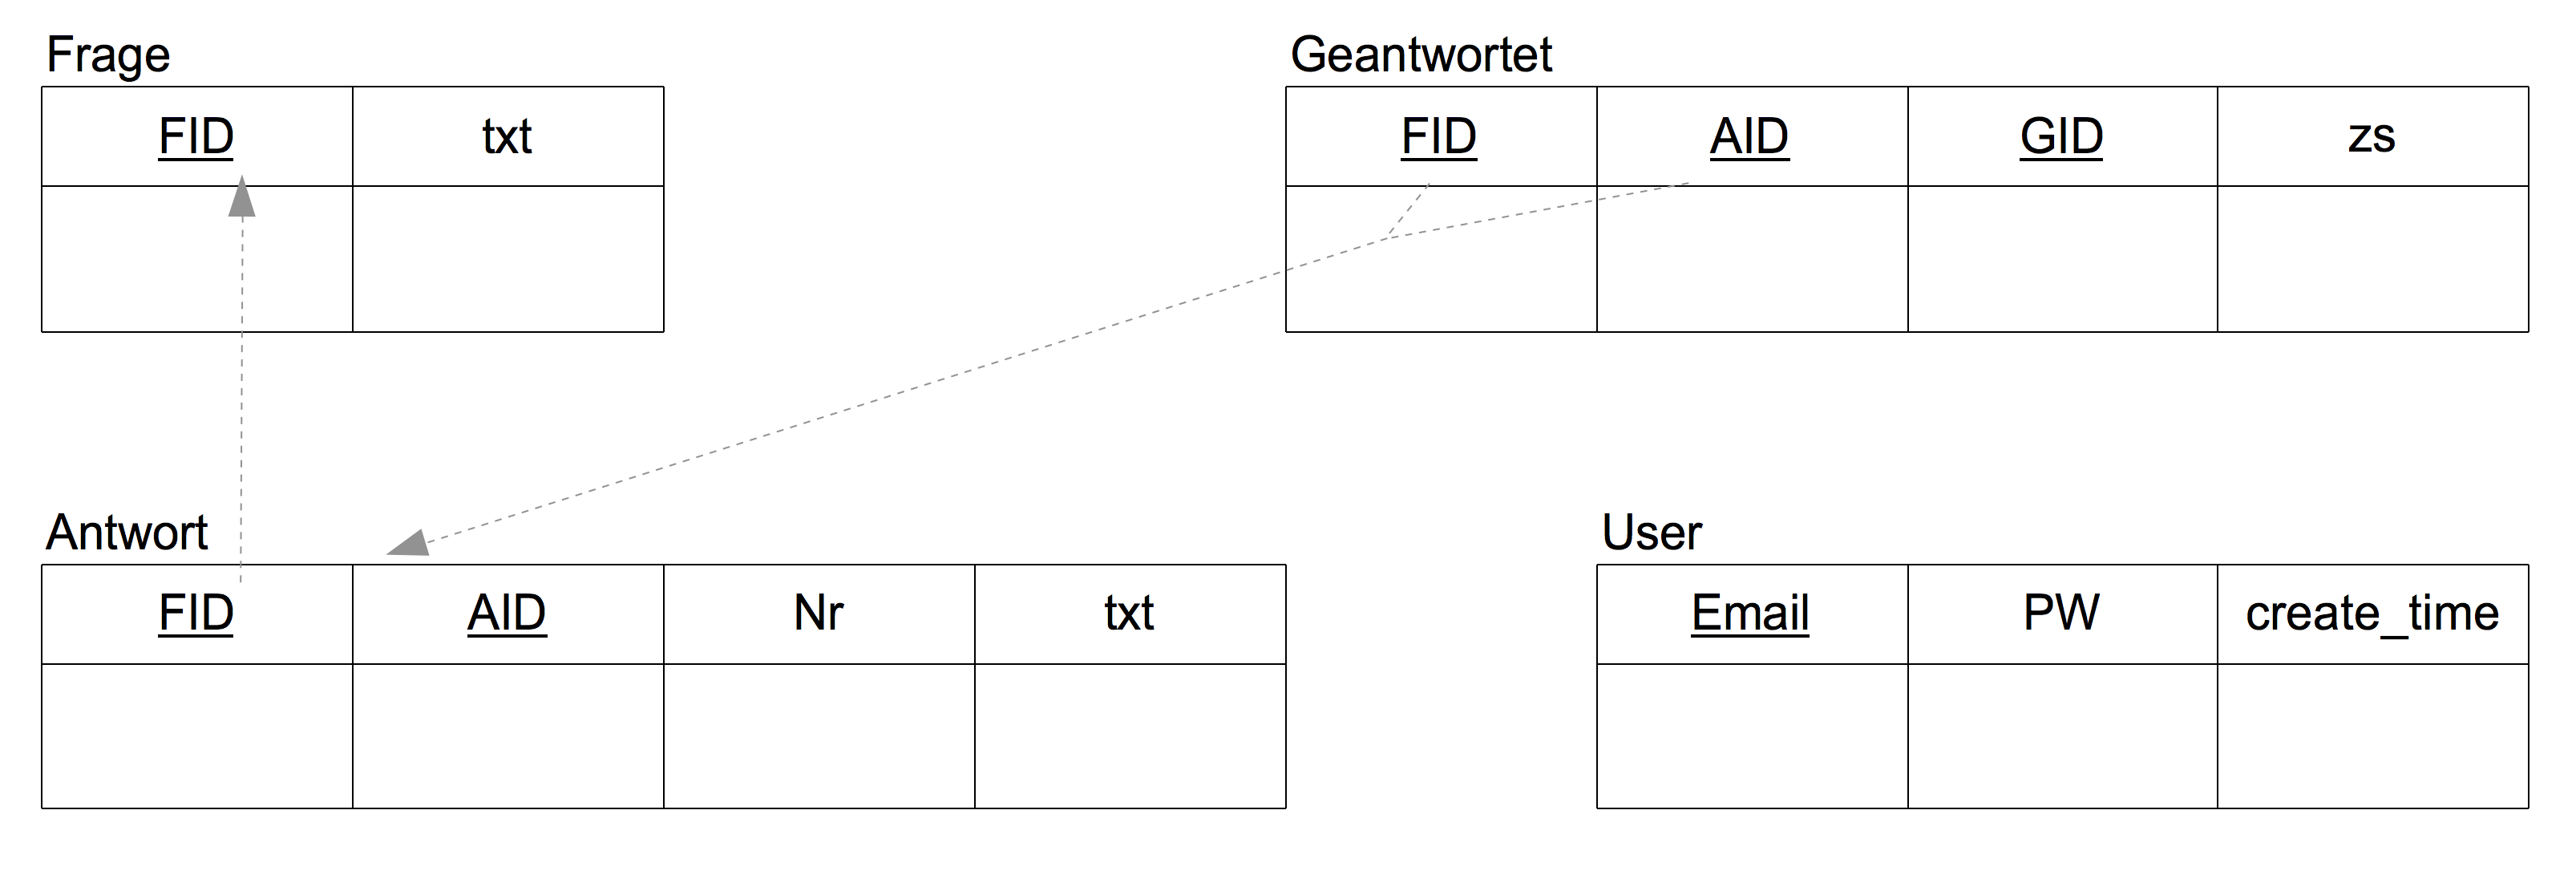
\includegraphics[width=\textwidth]{relmod.jpg}
\caption{Relationales Modell}
\end{center}
\label{fig:relmod}
\end{figure}

\subsection{Umsetzung in SQL}

\subsubsection{Tabelle: user --- Benutzerverwaltung}
\begin{figure}[H]
\begin{minted}[bgcolor=bg]{sql}
CREATE TABLE user (
  email VARCHAR(255) NOT NULL,
  pw CHAR(32) NOT NULL,
  create_time TIMESTAMP DEFAULT CURRENT_TIMESTAMP,
  PRIMARY KEY (`email`));
\end{minted}
\caption{SQL: CREATE TABLE user}
\label{sql:tbluser}
\end{figure}

Als Benutzername und auch als Primärschlüssel wird die E--Mail Adresse des Administrators genutzt. Da diese den Nutzer eindeutig identifiziert wird auf einen seperaten Nutzernamen und auch auf eine generierte ID als Primärschlüssel verzichtet.

Das Passwort sollte nicht im Klartext in der Datenbank gespeichert werden. Ein \code{salted hash}\footnote{Also der Hashwert des Passworts, welches zuvor mit Applikationsspezifischen Zusatzdaten ergänzt wurde} schützt hier das Passwort vor dem Ausspähen durch den Administrator selbst\footnote{Spätestens seit dem Datenklau bei Vodafone\footnote{\cite{vodafone}} eine dokumentierte Gefahr} oder durch Angreifer.\\
Die hier reservierten 32 Byte sind für den in der MySQL--Dokumentation\footnote{\cite{mysql-pcrypt}} emphohlenen MD5-Hash ausreichend. Da die entsprechende PHP--Dokumentation\footnote{\cite{php-pcrypt}} hier allerdings eine genau entgegengesetzte Empfehlung gibt, ist dieser Sicherheitsaspekt für ein Produktivsystem nochmals genauer zu prüfen.

\subsubsection{Tabelle: frage --- Fragestellungen}
\begin{figure}[H]
\begin{minted}[bgcolor=bg]{sql}
CREATE TABLE frage (
  fid INT NOT NULL AUTO_INCREMENT,
  txt VARCHAR(1024) NOT NULL,
  CONSTRAINT pk_frage PRIMARY KEY (`fid`));
\end{minted}
\caption{SQL: CREATE TABLE frage}
\label{sql:tblfrage}
\end{figure}

In der Tabelle „Frage“ wird lediglich der Text der Frage sowie die eindeutige Frage--ID gespeichert. Letztere dient als Primärschlüssel.

\subsubsection{Tabelle: antwort --- Antwortmöglichkeiten}
\begin{figure}[H]
\begin{minted}[bgcolor=bg]{sql}
CREATE TABLE antwort (
  fid INT NOT NULL, 
  aid INT NOT NULL AUTO_INCREMENT,
  nr  INT NULL,
  txt VARCHAR(1024) NOT NULL,
  CONSTRAINT pk_antwort PRIMARY KEY (fid, aid),
  CONSTRAINT fk_antwort_frage_fid FOREIGN KEY (fid) 
  REFERENCES frage(fid) 
  ON UPDATE CASCADE 
  ON DELETE CASCADE );
\end{minted}
\caption{SQL: CREATE TABLE antwort}
\label{sql:tblantwort}
\end{figure}

Aufgrund der Modellierung als schwache Entity setzt sich der Primärschlüssel der Tabelle „Antwort“ aus der Frage--ID sowie der Antwort--ID zusammen. Zusätzlich wird der Antworttext sowie eine frei zu vergebende Nummer gespeichert, welche für die Sortierreihenfolge bei der Anzeige genutzt werden kann.

Die Integritätsbedingung wird so definiert, dass beim Löschen einer Frage auch die zugehörigen Antwortmöglichkeiten gelöscht werden.

\subsubsection{Tabelle: geantwortet --- Gegebene Antworten}
\begin{figure}[H]
\begin{minted}[bgcolor=bg]{sql}
CREATE TABLE geantwortet (
  fid INT NOT NULL,
  aid INT NOT NULL,
  gid INT NOT NULL AUTO_INCREMENT,
  zs TIMESTAMP DEFAULT CURRENT_TIMESTAMP,
  CONSTRAINT pk_geantwortet PRIMARY KEY (fid, aid, gid),
  CONSTRAINT fk_geantwortet_antwort_aid FOREIGN KEY (fid, aid) 
  REFERENCES antwort(fid, aid) 
  ON UPDATE CASCADE 
  ON DELETE CASCADE );
\end{minted}
\caption{SQL: CREATE TABLE geantwortet}
\label{sql:tblgeantwortet}
\end{figure}

Für die Speicherung der gegebenen Antworten in der Tabelle „geantwortet“ genügt der aus Frage--ID, Antwort--ID und Geantwortet--ID zusammengesetzte Primärschlüssel. Zusätzlich wird noch der jeweilige Zeitstempel für spätere Auswertungen erfasst.

Auch hier stellt die Integritätsbedingung sicher, dass beim Wegfall der entsprechenden Antwortmöglichkeit keine undefinierten gegebene Antworten zurückbleiben.

\section{Klassenhierarchie}

Der Zugriff auf die in der bislang beschriebenen Datenbank gespeicherten Daten erfolgt über die folgende  Klassenhierarchie:

\begin{figure}[H]
\begin{center}
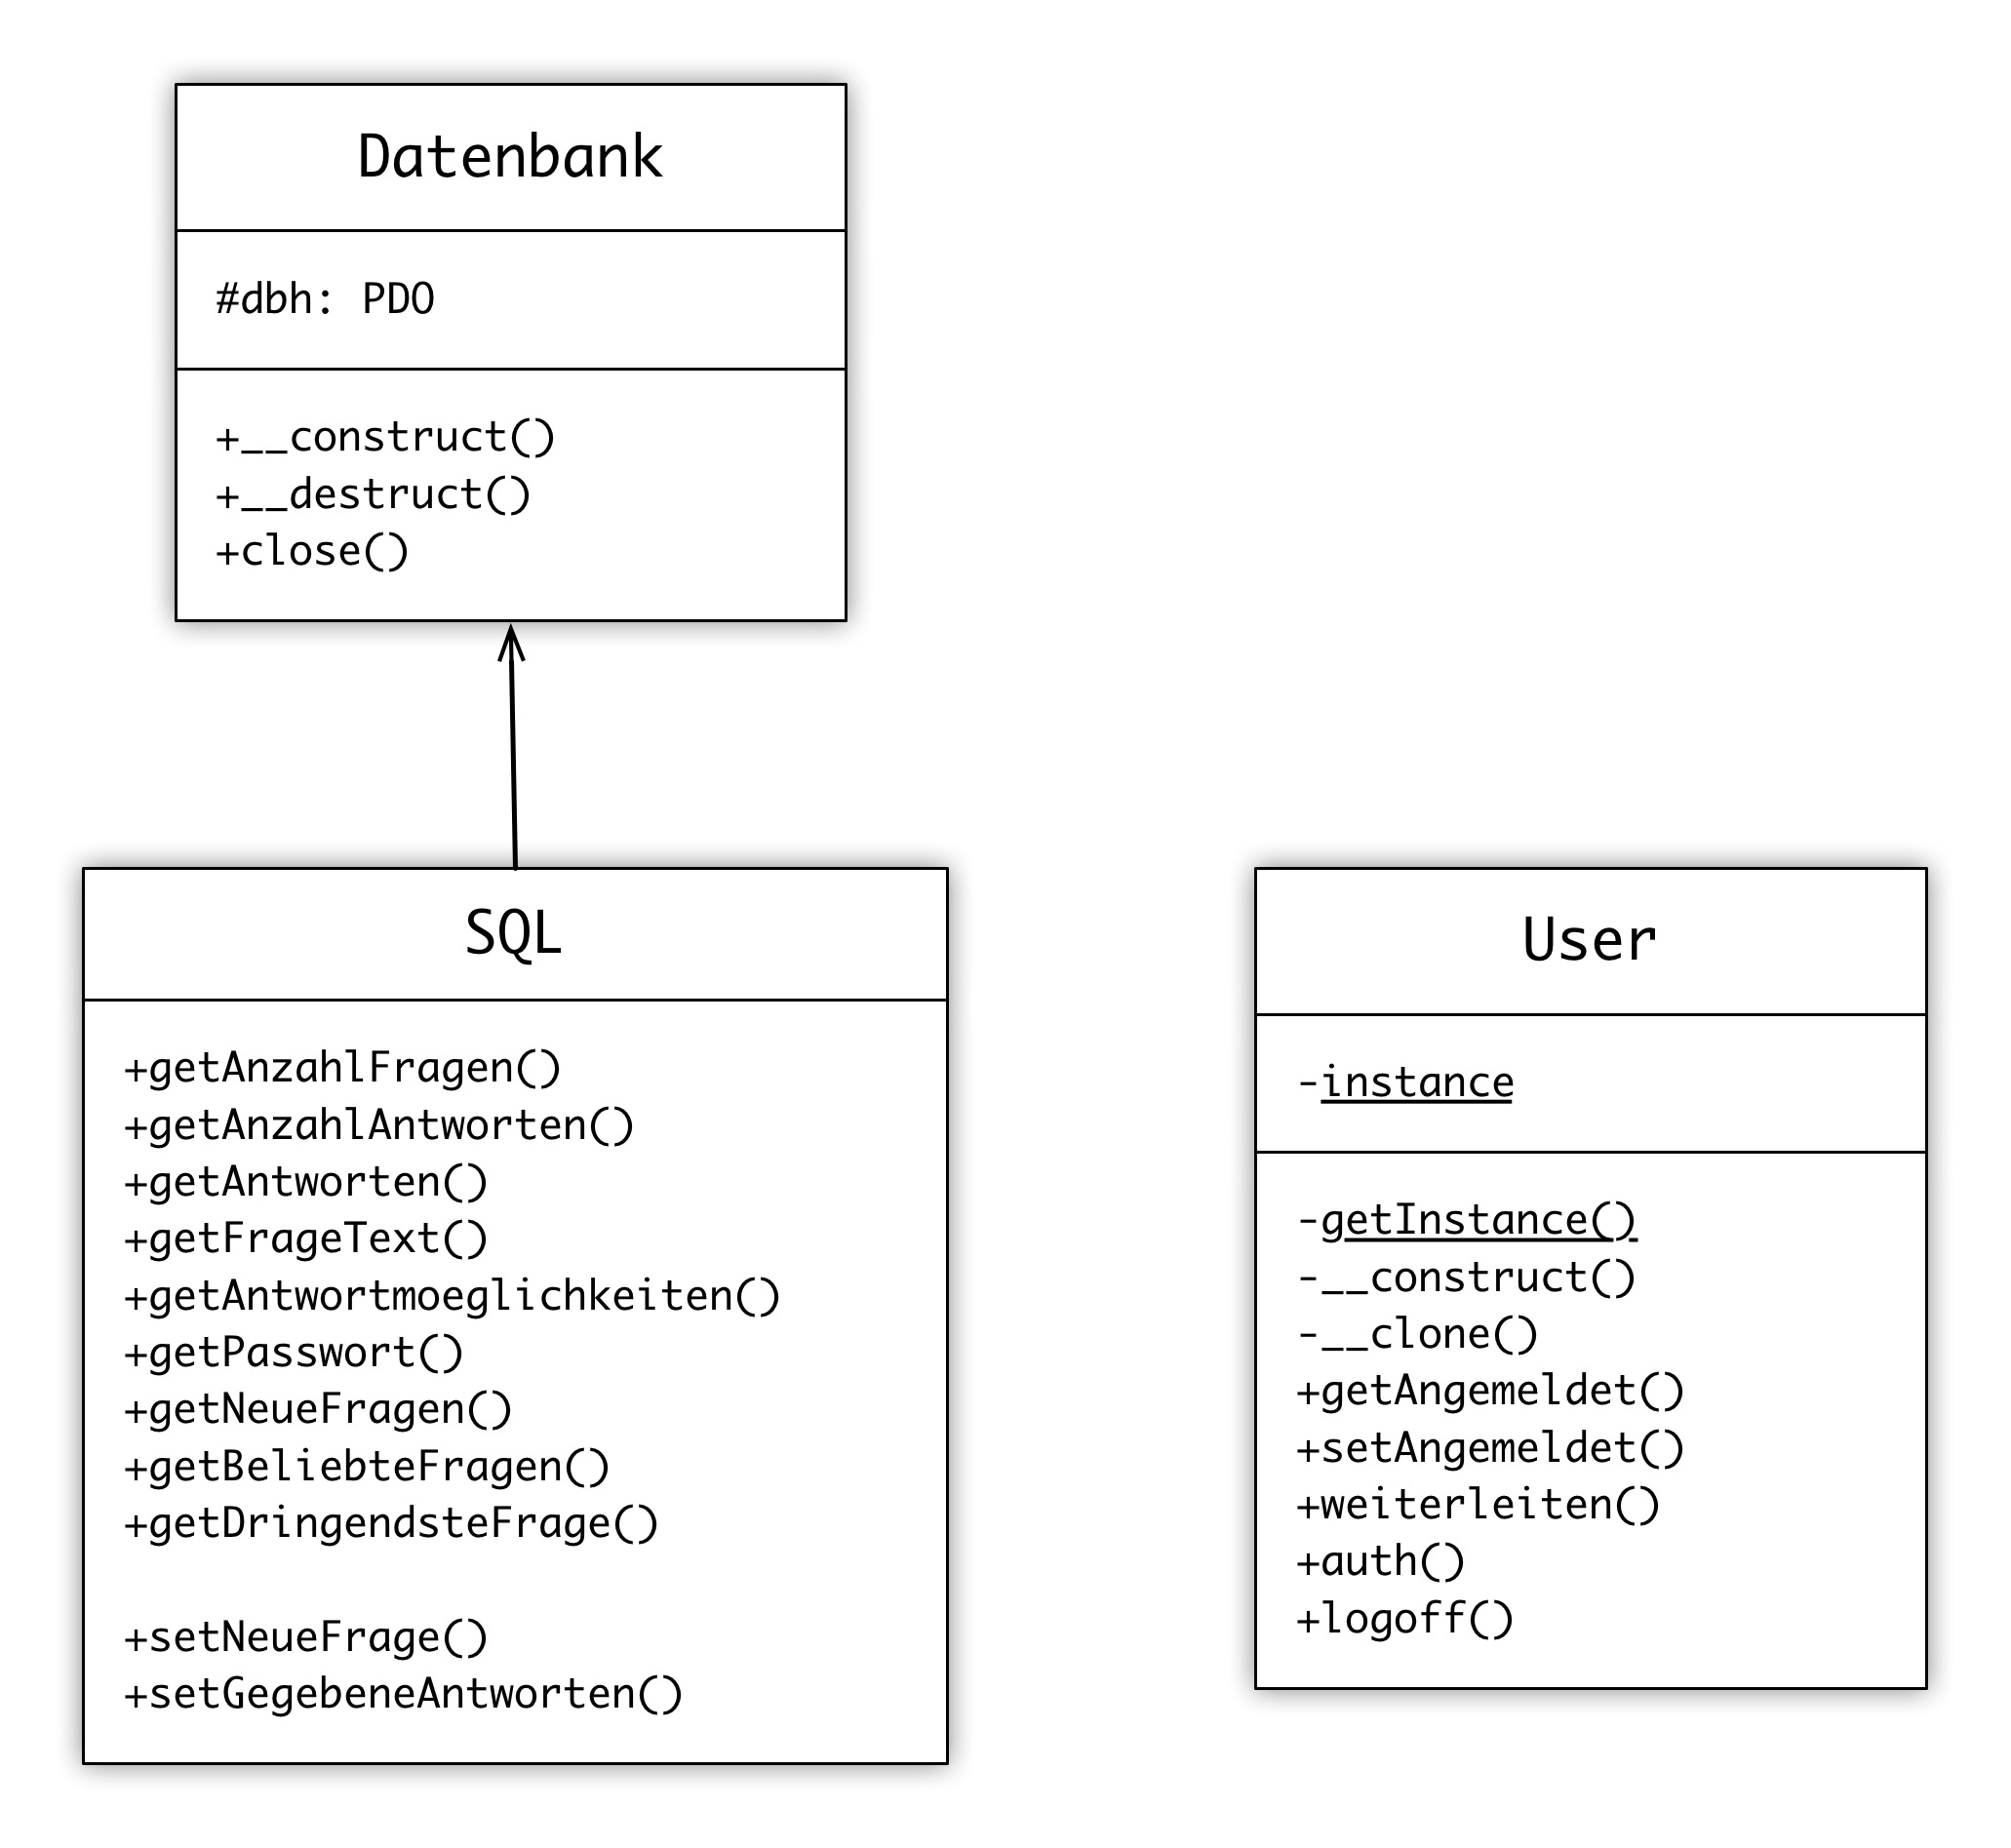
\includegraphics[width=\textwidth]{UML.jpg}
\caption{UML--Klassendiagramm}
\end{center}
\label{fig:uml}
\end{figure}

Die Implementation der Klassen ist im beigefügten Quelltext in den Dateien \code{.../class/Datenbank.php}, \code{.../class/SQL.php} und \code{.../class/User.php} zu betrachten. Auch die Klasse „User“ nutzt für den Datenbankzugriff die Klasse „SQL“. Dies geschieht allerdings nur innerhalb der Methode \code{auth()} über eine lokale Variable und ist daher im UML--Diagramm nicht zu erkennen.

\subsection{Klasse: Datenbank --- Low--Level Zugriff}

Die Klasse „Datenbank“ stellt die unterste Ebene des Datenzugriffs der Anwendung dar. Aufgrund der von PHP zur Verfügung gestellten PDO--Klasse greift jedoch auch diese Klasse nicht direkt auf die Datenbank  zu. Das PDO--Objekt ist als Attibut in der Klasse vorhanden. Die für den Zugriff notwendigen Angaben werden im Konstruktor aus der Konfigurationsdetails gelesen und anschließend wird die Verbindung zur Datenbank hergestellt. 

Die Datenbankverbindung bleibt so lange bestehen, wie die Instanz existiert. Ein Objekt mit geschlossener Datenbankverbindung würde die Notwendigkeit von zusätzlichen Fehlerprüfungen bzw. der erneuten Herstellung der Verbindung mit sich bringen. Um hierauf ausdrücklich hinzuweisen ist die Methode \code{close()} ohne Funktion definiert.
 
\subsection{Klasse: SQL --- High--Level Zugriff}

In der Klasse „SQL“ werden die SQL--Abfragen gekapselt. Der aufrufende PHP--Code benötigt keinerlei Wissen über die zu Grunde liegende Datenbank. Es müssen lediglich die Get-- und Set--Methoden eines Objektes vom Typ SQL aufgerufen werden. Innerhalb dieser Methoden werden dann die SQL--Abfragen mit Hilfe des geerbten PDO--Objekts vorbereitet und dann mit den geforderten Parametern aufgerufen. Die Ergebnisse werden dann als einzelner Wert oder als Objekt mit mehreren Werten bzw. Array zurückgegeben. Hierbei wird die jeweils geeignete Form gewählt.

Zum Speichern von neuen Fragen und Antwortmöglichkeiten bzw. von gegebenen Antworten werden diese an die entsprechenden Set--Methoden übergeben. Hierin werden die zum Abspeichern benötigten SQL-INSERTs in eine Transaktion verpackt. Somit ist auch bei gleichzeitigem Zugriff mehrerer Nutzer oder im Fehlerfall ein konsistenter Zustand des Datenbestandes gesichert.

Durch die Reduzierung der Aufrufe auf die passenden Get-- und Set--Methoden wird in der SQL-Klasse das Fassden-Entwurfsmuster realisiert. Der Aufrufende Code benötigt keinerlei Informationen über die Datenstruktur, die Datenbank oder Transaktionen. Änderungen an diesen technischen Details wirken sich lediglich auf die SQL--Klasse aus. So lange diese laut Spezifikation Werte entgegennimmt und zurückliefert, muss kein weiterer Programmcode geändert werden.

\subsubsection{Speichern von neuen Fragen und Antwortmöglichkeiten}

In der Methode \code{setNeueFrage()} werden neue Fragen und die zugehörigen Antwortmöglichkeiten in der Datenbank abgespeichert. Hierzu werden die entsprechenden Texte in den Parametern \code{\$fragetext} und \code{\$antworten} übergeben werden. Bei letzterem handelt es sich um ein Array, da es pro Frage mehrere Antwortmöglichkeiten gibt.

Das Datenbankschema verlangt es, dass zu jeder Antwortmöglichkeit die ID der zugehörigen Frage gespeichert wird. Somit wird zunächst die Frage in die Datenbank eingefügt. Die automatisch generierte ID kann dann mit der PDO--Methode \code{lastInsertId()} ausgelesen werden. Anschließend werden die Antwortmöglichkeiten in einer \code{foreach}--Schleife in die Datenbank eingefügt.

Dieser Vorgang besteht somit aus vielen einzelnen Schritten. Fehlermöglichkeiten bestehen im PHP--Code selbst sowie beim Zugriff auf die Datenbank. An jeder Stelle sind Unterbrechungen durch weitere Instanzen der Anwendung möglich, was im schlimmsten Fall zu einer inkorrekten Frage--ID führen könnte. Es ist sicher zu stellen, dass entweder die gesamte Kombination von Frage mit allen zugehörigen Antwortmöglichkeiten gespeichert wird, oder das Speichern gar nicht statt findet und mit einer entsprechenden Fehlermeldung abbricht. Im Fehlerfall darf keine Frage ohne den kompletten Antwortsatz in der Datenbank sein. 

Daher wird der gesamte Vorgang in einer SQL--Transaktion eingebettet und im Fehlerfall werden schon getätigte Änderungen mit einem Rollback zurückgenommen. Somit ist Konsistenz der Datenbank zu jedem Zeitpunkt sichergestellt.

\subsection{Klasse: User --- Benutzerverwaltung}

Die Benutzerverwaltung nutzt das Singleton Entwurfsmuster. Dieses wird durch die folgenden Maßnahmen implementiert: Die private Deklaration des Konstruktors sowie der \code{clone()} Methode wird die direkte Instanziierung der Klasse unterbunden. Eine Referenz auf die Instanz wird in der ebenfalls privaten statischen Variable \code{ \$instance } gespeichert und über die öffentliche Funktion \code{getInstance()} bekannt gemacht.

Die Funktion \code{auth()} erwartet als Parameter den Benutzernamen und das Passwort sowie optional eine URL zu der im Falle der erfolgreichen Authentifizierung umgeleitet werden soll. Der Datenbankzugriff erfolgt über eine lokale Instanz der Klasse SQL. Stimmen die Anmeldedetails mit den in der Datenbank gespeicherten überein werden in der von PHP zur Verfügung gestellten \code{\$\_SESSION}--Variable das Feld „angemeldet“ mit \code{TRUE} und das Feld „benutzer“ mit dem Benutzernamen gefüllt. Stimmen die Anmeldedaten nicht mit den gespeicherten Werten überein, so erhält das Feld „angemeldet“ den Wert \code{FALSE}.

Die Funktion \code{logoff()} meldet den momentan anfemeldeten Nutzer ab, in dem die Session-Variable zerstört und damit auch die Felder „angemeldet“ und „benutzer“ löscht.

Die Funktion \code{setAngemeldet()} ist eine private Hilfsmethode, mit der das Feld „angemeldet“ der \code{\$\_SESSION}--Variable gesetzt werden kann. Da sie aus der Methode \code{getInstance()} heraus aufgerufen wird, ist sie wie diese auch statisch deklariert.

Die Funktion \code{getAngemeldet()} dient zur Anfrage des Anmeldestatus. Sie wird immer dann aus der Anwendung heraus aufgerufen, wenn der Seitenaufbau für angemeldete Benutzer anders sein soll, wie für nicht angemeldete. Am auffällisten ist dies beim Aufruf der Seite zur Eingabe von neuen Fragen. Hier wird dem nicht angemeldeten Nutzer das Login--Formular angezeigt, wärend dem angemeldeten Nutzer die gewünschte Funktion direkt zur Verfügung steht.\\
Aber auch in Details können sich die Seiten unterscheiden: Die in der Seitenleiste angebotenen Links können schon entsprechend angepasst sein. Auf diese Weise werden dem Nutzer nur die Möglichkeiten gezeigt, die für ihn tatsächlich relevant sind. 

\section{Seitenstruktur}

\begin{figure}[H]
\begin{center}
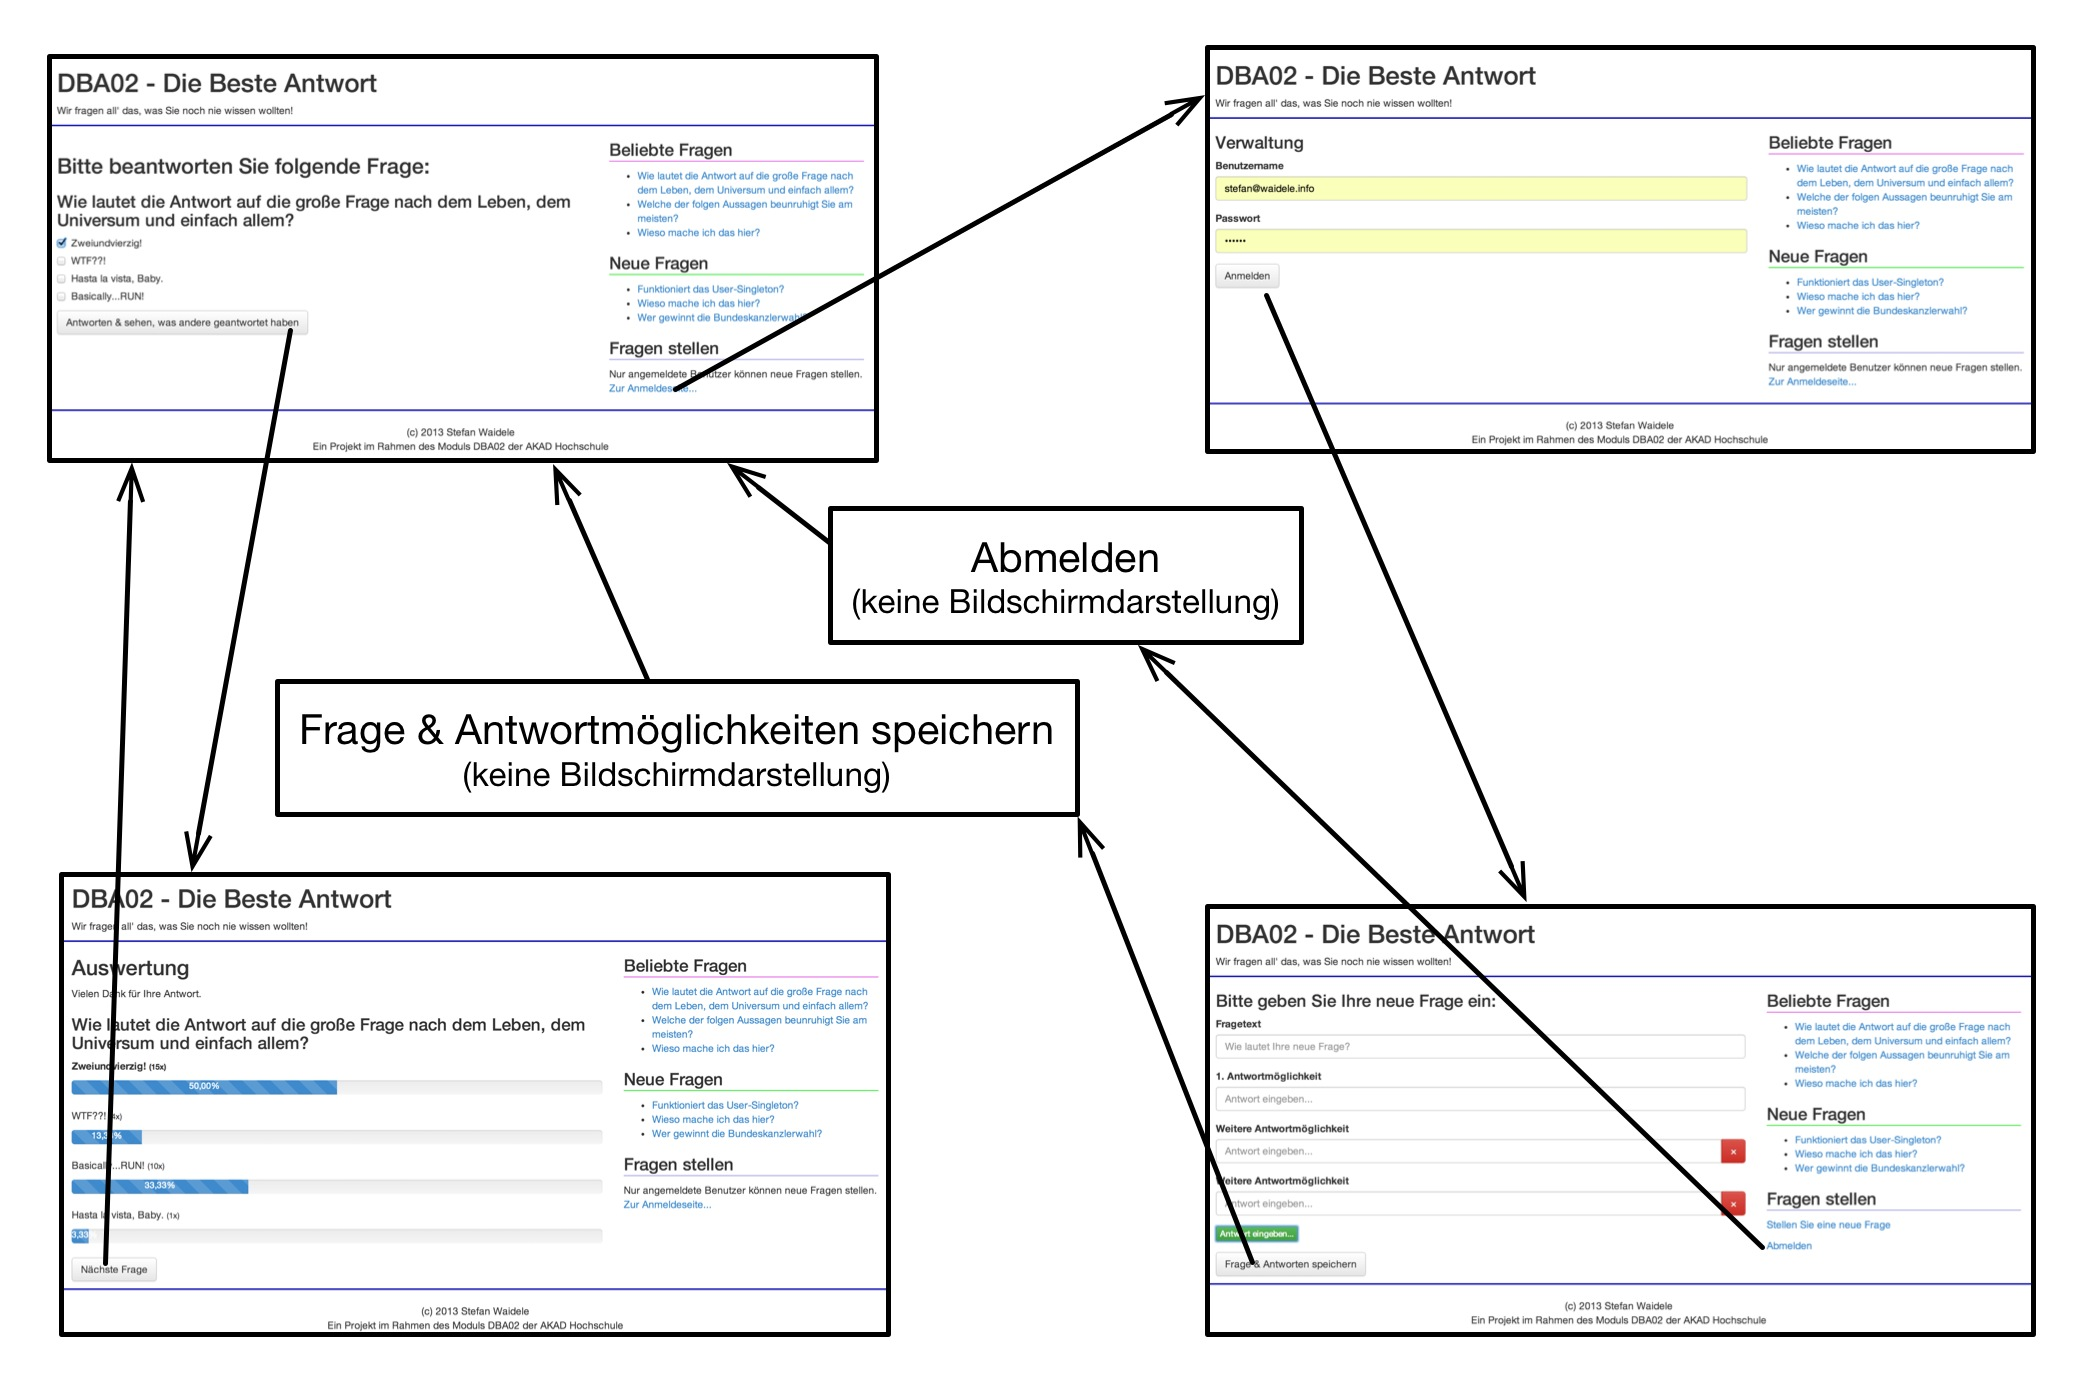
\includegraphics[width=\textwidth]{zustaende.jpg}
\caption{HTML--Seiten und Verlinkungen}
\end{center}
\label{fig:zustaende}
\end{figure}

